\section{Orthogonal Matching Pursuit}
\label{JM:sec:GOMP}

In the following section, preconditioned generalized orthogonal matching pursuit (GOMP) \cite{JMTongEtAl2020} will be implemented.
Matching pursuit algorithms are a class of greedy algorithms designed to solve the sparse signal recovery problem

\begin{equation}
\begin{aligned}
    \min_x \quad & \left\lVert x \right\rVert_0 \\
    \textrm{s.t.} \quad & y = \Psi x
\end{aligned}
\end{equation}

where $x \in \mathbb{R}^n$ represents an unknown, $K$ sparse basis for a signal $y \in \mathbb{R}^m$ in $\Psi \in \mathbb{R}^{m \times n}$, also called the sampling matrix.
This is done by iteratively reducing the estimation error of the recovered signal by selecting $S$ most similar, new components from the sampling matrix.\\

The main algorithm can be described as follows

\begin{algorithm}[H]
    \SetAlgoLined
    \KwResult{$x$}
    \KwData{$y$, $\Psi$, $K$, $S = 1$}
    Projection onto span\; 
    $P = \Psi^T \left(\Psi\Psi^T\right)$;
    $\tilde{y} = P y$;
    $\tilde{\Psi} = P \Psi$\;
    Initialize residual and support\;
    $r = y$;
    $\Lambda = \emptyset$\;
    \While{Not converged}{
        $\Omega = \delta_S\left( \left| \tilde{\Psi}^T~r \right| \right)$\;
        $\Lambda = \Lambda \cup \Omega$\;
        $x = \min \left\lVert \tilde{y} - \tilde{\Psi}u \right\rVert_2~, \quad supp(u) = \Lambda$\;
        $r = \tilde{y} - \tilde{\Psi} x$\;
    };
\end{algorithm}

Here $\delta_S\left( x \right) : \mathbb{R}^n \mapsto \lbrace 0, 1 \rbrace^n$ denotes (with abuse of notation) the mapping of the $S$ largest elements onto a corresponding
indicator vector. A similar notation to the pseudocode above can be achieved in \textit{Julia}. For brevity, only necessary elements of the source code will be shown, which can be found in detail in REF. The function is defined as follows

\lstinputlisting[language=Julia,firstline=4, lastline=6]{../scripts/gomp.jl}

First, we will focus on the preconditioning via the matrix $P \in \mathbb{R}^{m \times m}$ mapping onto the
column span of $\Psi$

\lstinputlisting[language=Julia,firstline=22, lastline=26]{../scripts/gomp.jl}

Next, the iterative computation of the support, corresponding coefficients and residuals is performed

\lstinputlisting[language=Julia,firstline=37, lastline=50]{../scripts/gomp.jl}

As can be seen from above, the implementation is quite similar to its mathematical counterpart, enhancing the interpretability and readability. 
The results of the algorithm are shown in Fig. \ref{JM:fig:GOMP}, where a 100 dimensional sparse vector $x$ has been recovered.

\begin{figure}
    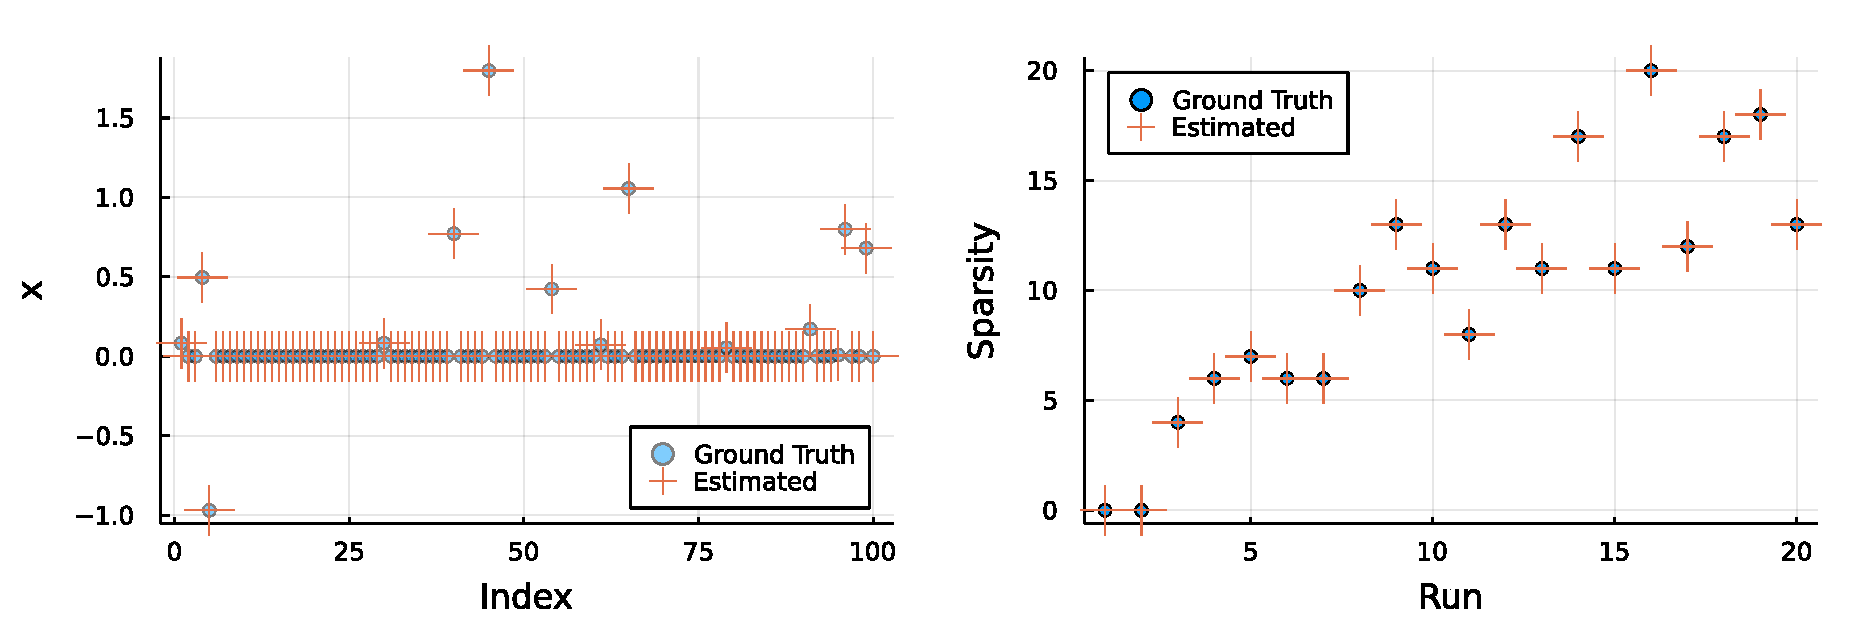
\includegraphics[width = 0.9\textwidth]{../figures/merged.pdf}
    \caption{Performance of GOMP for a single sparse 100 dimensional vector (left) and with different sparsities (right). The signal $y$ is of dimension 300 and has been generated by a random dense sampling matrix.
    GOMP has been used with $K=50, S=1$ and run for at most 100 iterations with a absolute tolerance $\epsilon = 0.1$.}
    \label{JM:fig:GOMP}
\end{figure}

\newpage